\documentclass{beamer}

\usetheme{CambridgeUS}
\usecolortheme{orchid}

\usepackage{wrapfig}
\usepackage{siunitx}
\usepackage{inconsolata}
\usepackage{amsmath}
\usepackage{bm}
\usepackage{adjustbox}
\usepackage{nicefrac}

% Tikz
\usepackage{tikz}
\usetikzlibrary{positioning,shapes,arrows,calc,intersections}
\usepackage{pgfplots}
\usepgfplotslibrary{dateplot}
\pgfplotsset{compat=1.8}

\input{custom}

\begin{document}

\title[Reduced Basis Methods]{
  Spline-based Compatible Reduced Basis Methods for Flow Problems
}
\author[E. Fonn]{
  E.~Fonn\inst{1,2} \and
  E.~H.~van Brummelen\inst{3} \and
  T.~Kvamsdal\inst{4} \and
  A.~Rasheed\inst{2}
}
\institute[SINTEF]{
  \inst{1}%
  \url{eivind.fonn@sintef.no}
  \and \inst{2}%
  Applied Mathematics, SINTEF ICT
  \and \inst{3}%
  Department of Mechanical Engineering, TU/e
  \and \inst{4}%
  Department of Mathematical Sciences, NTNU
}
\date[IGA 2017]{}

\definecolor{darkblue}{HTML}{00688B}
\definecolor{darkgreen}{HTML}{6E8B3D}
\definecolor{cadet}{HTML}{DAE1FF}
\definecolor{salmon}{HTML}{FFB08A}

\titlegraphic{\includegraphics[width=0.3\textwidth]{figs/sintef}}

\begin{frame}
  \titlepage
\end{frame}

\begin{frame}
  \frametitle{Outline}
  \begin{enumerate}
  \item Basic idea of ROM
  \item ROM in practice
  \item Backwards-facing step channel
  \item Divergence-free function spaces
  \end{enumerate}
\end{frame}

\begin{frame}
  \frametitle{Reduced order modelling}
  \begin{itemize}
  \item We are interested generating solutions $\bm u(\bm \mu)$ to a physical
    model that depend on a set of pre-determined \emph{parameters},
    $\bm\mu \in \mathcal{P}$.
  \item In many cases, the computational cost of such a solution is prohibitive,
    especially in applications where repeated sampling of the parameter space is
    necessary (optimization, control, etc.)
  \item This cost is tied to the number of degrees of freedom required to
    accurately represent solutions.
  \end{itemize}
\end{frame}

\begin{frame}
  \frametitle{Reduced order modelling}
  \begin{itemize}
  \item Usually, the practical dimension $M$ of the solution space
    \[ \left\{ \bm u(\bm \mu) \,|\, \bm \mu \in \mathcal{P} \right\}\]
    is much lower than the number $N$ of DoFs needed by conventional methods.
  \item Idea: create a model whose internal dimension closely matches the
    physical dimension of the problem.
  \item In many cases, such a model will have less than $100$ degrees of
    freedom, allowing extremely fast solutions.
  \end{itemize}
\end{frame}

\begin{frame}
  \frametitle{Reduced order modelling}
  \begin{itemize}
  \item Given a high-fidelity model, create a basis consisting of solutions to
    that model. (This requires a number of high-fidelity samples, called an
    \emph{ensemble}.)
  \item In practice, partial orthogonal decomposition is applied to the ensemble
    before choosing the basis. This has the effect of
    \begin{itemize}
    \item orthogonalizing the basis, controlling the condition number, and
    \item ranking basis functions by ``importance'' (feature extraction).
    \end{itemize}
  \item Then, given a basis $\bm V$ (a tall matrix), the reduced form of

    \[
      \bm A(\bm \mu) \bm u(\bm \mu) = \bm f(\bm \mu)
    \]
    is
    \[
      \left( \bm V^\intercal \bm A(\bm \mu) \bm V \right) \bm u_M (\bm \mu)
      = \bm V^\intercal \bm f(\bm \mu)
    \]
  \end{itemize}
\end{frame}

\begin{frame}
  \frametitle{ROM in practice}
  \begin{itemize}
  \item It is vital to understand the precise relationship between the
    parameters and the system.
  \item Given a system $\bm A(\bm \mu) \bm u(\bm \mu) = \bm f(\bm \mu)$, we seek
    an \emph{affine representation} of the form (possibly approximate)
    \[
      \bm A(\bm \mu) = \sum_i \xi_i(\bm \mu) \bm A_i, \qquad
      \bm f(\bm \mu) = \sum_i \chi_i(\bm \mu) \bm f_i
    \]
    This facilitates fast ``reduced assembly,'' i.e.
    \[
      \bm V^\intercal \bm A(\bm \mu) \bm V =
      \sum_i \xi_i(\bm \mu)
      \underbrace{\bm V^\intercal \bm A_i \bm V}_{\text{precompute}}
    \]
  \end{itemize}
\end{frame}

% \begin{frame}
%   \frametitle{ROM in practice}
%   \begin{figure}
%     \begin{center}
%       \begin{tikzpicture}[
%         block/.style={
%           minimum width=40mm,
%           text width=38mm,
%           align=center,
%           rounded corners=1mm,
%         },
%         offline/.style={
%           block,
%           draw=darkblue,
%           fill=cadet,
%         },
%         online/.style={
%           block,
%           draw=darkblue,
%           fill=salmon,
%         },
%         clear/.style={
%           block,
%           draw=darkblue,
%         },
%         ]
%         \node[offline] (pde) {\tiny Parametrized PDE};
%         \node[offline, below=2mm of pde] (hifi) {
%           \tiny
%           High-fidelity discr. \\[0.5mm]
%           $\bm A_h(\bm \mu) \bm u_h(\bm \mu) = \bm f_h(\bm \mu)$ \\[0.5mm]
%           $\begin{aligned}
%             \bm A &= \textstyle \sum_i \xi_i(\bm \mu) \bm A_i \\
%             \bm f &= \textstyle \sum_i \chi_i(\bm \mu) \bm f_i
%           \end{aligned}$
%         };
%         \node[offline, below=2mm of hifi] (snaps) {
%           \tiny
%           Generate a RB by applying POD to snapshot solutions, and construct
%           projection matrix $\bm V$ \par
%         };
%         \node[offline, below=2mm of snaps] (proj) {
%           \tiny
%           Projection \\[1.0mm]
%           $\begin{aligned}
%             \bm A^M_i &= \bm V^\intercal \bm A_i \bm V \\
%             \bm f^M_i &= \bm V^\intercal \bm f_i
%           \end{aligned}$
%         };
%         \node[online, right=9mm of pde] (mu) {\tiny $\bm \mu$};
%         \node[online, below=2mm of mu] (asm) {
%           \tiny
%           RB system assembly \\[1.0mm]
%           $\begin{aligned}
%             \bm A_M &= \textstyle \sum_i \xi_q(\bm \mu) \bm A^M_i \\
%             \bm f_M &= \textstyle \sum_i \chi_q(\bm \mu) \bm f^M_i
%           \end{aligned}$
%         };
%         \node[online, below=2mm of asm] (sol) {
%           \tiny
%           RB system solution \\[0.0mm]
%           $\bm A_M(\bm \mu) \bm u_M(\bm \mu) = \bm f_M(\bm \mu)$
%         };
%         \node[clear, below=2mm of sol] (err) {
%           \tiny
%           Error estimate \\[0.0mm]
%           $\| \bm u(\bm \mu) - \bm V \bm u_M(\bm \mu) \|$
%         };
%         \node[clear, below=2mm of err] (rec) {
%           \tiny
%           Recovery, visualization and post-processing \\[0.0mm]
%           $\bm u_M^h(\bm \mu) = \bm V \bm u_M(\bm \mu)$
%         };
%         \node[clear, below=2mm of rec] (eval) {
%           \tiny
%           Evaluating functionals of interest
%         };

%         \draw[->] (pde.south) -- (hifi.north);
%         \draw[->] (hifi.south) -- (snaps.north);
%         \draw[->] (snaps.south) -- (proj.north);
%         \draw[->] (mu.south) -- (asm.north);
%         \draw[->] (proj.east) -- ($(proj.east) + (3mm,0)$) -- ($(asm.west) - (6mm,0)$) -- (asm.west);
%         \draw[->] (asm.south) -- (sol.north);
%         \draw[->] (sol.west) -- ($(sol.west) - (3mm,0)$) -- ($(eval.west) - (3mm,0)$) -- (eval.west);
%         \draw[->] ($(err.west) - (3mm,0)$) -- (err.west);
%         \draw[->] ($(rec.west) - (3mm,0)$) -- (rec.west);
%       \end{tikzpicture}
%     \end{center}
%   \end{figure}
% \end{frame}

% \begin{frame}
%   \frametitle{Parameters}
%   \begin{itemize}
%   \item Spatially dependent parameters, e.g.~thermal diffusivity
%     $\bm\kappa(\bm x; \bm \mu)$ can be dealt with so long as they admit
%     an affine representation of the same type,
%     \[
%       \bm \kappa(\bm x; \bm \mu) =
%       \sum_i \theta_i(\bm \mu) \bm \kappa_i(\bm x).
%     \]
%   \item Parameter-dependent geometries can be dealt with by representing the
%     system on a reference geometry. The mapping should admit the same affine
%     representation.
%   \end{itemize}
% \end{frame}

\begin{frame}
  \frametitle{ROM in practice}
  \begin{itemize}
  \item Parameters must enter the system via terms that admit such a
    representation.
  \item Paremeter-dependent geometries can be dealt with by formulating the
    problem on a reference geometry.
  \item Non-homogeneous Dirichlet boundary conditions must be represented with
    lift functions $\bm \ell$.
  \item The reduced basis should represent the solution minus the lift, so that
    it satisfies homogeneous Dirichlet boundary conditions by linearity.
  \item Boundary conditions may also be parameter-dependent so long as the lift
    function admits the now familiar representation
    \[
      \bm \ell(\bm x; \bm \mu) =
      \sum_i \theta_i(\bm \mu) \bm \ell_i(\bm x).
    \]
  \end{itemize}
\end{frame}

\begin{frame}
  \frametitle{The backwards-facing step channel}
  \begin{center}
    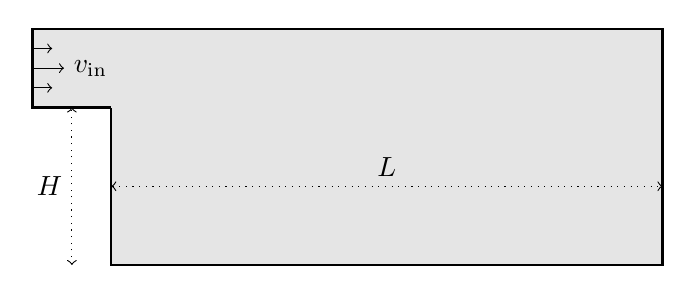
\begin{tikzpicture}
      \draw[thick, solid, fill=black!10]
      (0,0) -- (-1,0) -- (-1,1) -- (7,1) -- (7,-2) -- (0,-2) -- (0,0);
      \draw[<->, dotted] (0,-1) -- node[above,midway] {$L$} (7,-1);
      \draw[<->, dotted] (-0.5,-2) -- node[left,midway] {$H$} (-0.5,0);
      \draw[->] (-1,0.75) -- (-0.75,0.75);
      \draw[->] (-1,0.5) -- (-0.6,0.5);
      \draw[->] (-1,0.25) -- (-0.75,0.25);
      \node[anchor=west] at (-0.6,0.5) {$v_\text{in}$};
    \end{tikzpicture}
    \\~\\
    Figure: Problem domain with parameters. Additionally, the fluid viscosity
    $\nu$ is also a parameter. (See Quarteroni et.~al.~for more information.)
  \end{center}
\end{frame}

\begin{frame}
  \frametitle{The backwards-facing step channel}
  \begin{center}
    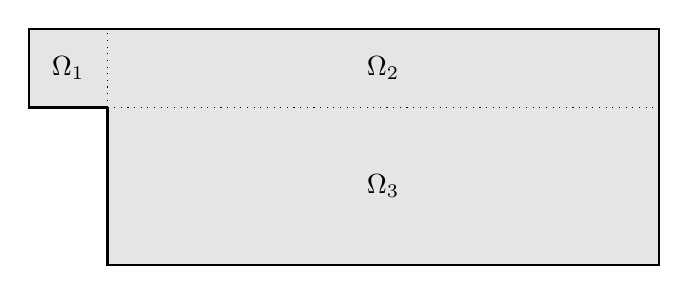
\begin{tikzpicture}
      \draw[thick, solid, fill=black!10]
      (0,0) -- (-1,0) -- (-1,1) -- (7,1) -- (7,-2) -- (0,-2) -- (0,0);
      \draw[dotted] (0,0) -- (7,0);
      \draw[dotted] (0,0) -- (0,1);
      \node at (-0.5,0.5) {$\Omega_1$};
      \node at (3.5,0.5) {$\Omega_2$};
      \node at (3.5,-1) {$\Omega_3$};
    \end{tikzpicture}
    \\~\\
    Figure: Multipatch decomposition and subdomains.
  \end{center}
\end{frame}

\begin{frame}
  \frametitle{The backwards-facing step channel}
  \begin{center}
    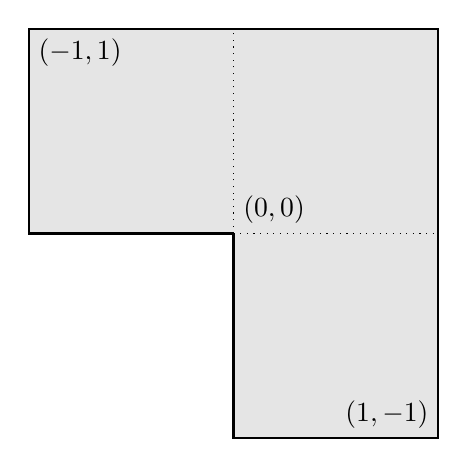
\begin{tikzpicture}[scale=2.6]
      \draw[thick, solid, fill=black!10]
      (0,0) -- (-1,0) -- (-1,1) -- (1,1) -- (1,-1) -- (0,-1) -- (0,0);
      \draw[dotted] (0,0) -- (1,0);
      \draw[dotted] (0,0) -- (0,1);
      \node[anchor=south west] at (0,0) {$(0,0)$};
      \node[anchor=north west] at (-1,1) {$(-1,1)$};
      \node[anchor=south east] at (1,-1) {$(1,-1)$};
    \end{tikzpicture}
    \\~\\
    Figure: Reference geometry.
  \end{center}
\end{frame}

\begin{frame}
  \frametitle{Affine representation (examples)}
  \begin{align*}
    \nu \int_{\Omega(\bm \mu)} \nabla \bm v : \nabla \bm w
    &= \nu \int_{\hat{\Omega}_1} \hat{\nabla} \bm v : \hat{\nabla} \bm w \\
    &+ \frac{\nu}{L} \int_{\hat{\Omega}_2} \partial_{\hat{x}} \bm v \cdot \partial_{\hat{x}} \bm w
      + \nu L \int_{\hat{\Omega}_2} \partial_{\hat{y}} \bm v \cdot \partial_{\hat{y}} \bm w \\
    &+ \frac{\nu H}{L} \int_{\hat{\Omega}_3} \partial_{\hat{x}} \bm v \cdot \partial_{\hat{x}} \bm w
      + \frac{\nu L}{H} \int_{\hat{\Omega}_3} \partial_{\hat{y}} \bm v \cdot \partial_{\hat{y}} \bm w
  \end{align*}
\end{frame}

\begin{frame}
  \frametitle{Affine representation (examples)}
  \begin{align*}
    \int_{\Omega(\bm \mu)} (\bm u \cdot \nabla) \bm v \cdot \bm w
    &= \int_{\hat{\Omega}_1} (\bm u \cdot \hat{\nabla}) \bm v \cdot \bm w \\
    &+ \int_{\hat{\Omega}_2} (u_{x} \partial_{\hat{x}}) \bm v \cdot \bm w
      + H \int_{\hat{\Omega}_3} (u_{x} \partial_{\hat{x}}) \bm v \cdot \bm w \\
    &+ L \int_{\hat{\Omega}_2 \cup \hat{\Omega}_3}
      (u_{y} \partial_{\hat{y}}) \bm v \cdot \bm w
  \end{align*}
  \begin{align*}
    \ell_x(\hat{x}, \hat{y}) &= \begin{cases}
      \frac{v_\text{in}}{4} \hat{y}(1-\hat{y}), & \hat{y} > 0 \\
      0, & \hat{y} \leq 0,
    \end{cases} \\
    \ell_y &= 0.
  \end{align*}
\end{frame}

\begin{frame}
  \frametitle{The backwards-facing step channel (N-S spectrum)}
  \begin{center}
    \begin{tikzpicture}
      \begin{axis}[
        xlabel={$k$},
        ylabel={$\lambda_k$},
        ymode=log,
        width=0.9\textwidth,
        height=0.5\textwidth,
        grid=both,
        axis lines=left,
        legend style={
          font=\scriptsize,
          at={(1, 1)},
          anchor=north east,
        },
        ]
        \addplot[red, thick]
        table[x index={0}, y index={1}]{data/spectrum-ns-bs.csv};
        \addplot[blue, thick]
        table[x index={0}, y index={2}]{data/spectrum-ns-bs.csv};
        \legend{Velocity, Pressure};
        \only<2>{
          \draw[red, very thick, rounded corners=0.5mm] (1,8) rectangle (120,-40);
        }
        \only<3>{
          \draw[blue, very thick, rounded corners=0.5mm] (1,8) rectangle (100,-40);
        }
      \end{axis}
    \end{tikzpicture}
    \only<1>{
      Spectrum of velocity and pressure solutions.
    }
    \only<2>{
      There are about 120 unique velocity DoFs, \ldots
    }
    \only<3>{
      \ldots and about 100 unique pressure DoFs.
    }
  \end{center}
\end{frame}

\begin{frame}
  \only<1>{\frametitle{Backwards-facing step channel basis functions (1)}}
  \only<2>{\frametitle{Backwards-facing step channel basis functions (2)}}
  \only<3>{\frametitle{Backwards-facing step channel basis functions (3)}}
  \only<4>{\frametitle{Backwards-facing step channel basis functions (4)}}
  \only<5>{\frametitle{Backwards-facing step channel basis functions (5)}}
  \only<6>{\frametitle{Backwards-facing step channel basis functions (6)}}
  \begin{center}
    \only<1>{
      \adjustbox{trim={0.1\width} {0.0\height} {0.01\width} {0.0\height}, clip}{
        \includegraphics[width=1.2\textwidth]{figs/bfun-v000}
      }
    }
    \only<2>{
      \adjustbox{trim={0.1\width} {0.0\height} {0.01\width} {0.0\height}, clip}{
        \includegraphics[width=1.2\textwidth]{figs/bfun-v001}
      }
    }
    \only<3>{
      \adjustbox{trim={0.1\width} {0.0\height} {0.01\width} {0.0\height}, clip}{
        \includegraphics[width=1.2\textwidth]{figs/bfun-v002}
      }
    }
    \only<4>{
      \adjustbox{trim={0.1\width} {0.0\height} {0.01\width} {0.0\height}, clip}{
        \includegraphics[width=1.2\textwidth]{figs/bfun-v003}
      }
    }
    \only<5>{
      \adjustbox{trim={0.1\width} {0.0\height} {0.01\width} {0.0\height}, clip}{
        \includegraphics[width=1.2\textwidth]{figs/bfun-v004}
      }
    }
    \only<6>{
      \adjustbox{trim={0.1\width} {0.0\height} {0.01\width} {0.0\height}, clip}{
        \includegraphics[width=1.2\textwidth]{figs/bfun-v005}
      }
    }
    \only<1>{
      The first basis function closely mimics the mean velocity solution minus
      the lift. Its shape therefore heavily depends on the lift function used.
    }
    \only<2-5>{
      Subsequent basis functions represent significant features in order of
      importance.
    }
    \only<6>{
      The higher order basis functions show more erratic behaviour, features
      that are less important.
    }
  \end{center}
\end{frame}

\begin{frame}
  \frametitle{The backwards-facing step channel (Navier-Stokes)}
  \begin{center}
    \only<1>{
      \adjustbox{trim={0.1\width} {0.0\height} {0.1\width} {0.0\height}, clip}{
        \includegraphics[width=1.3\textwidth]{figs/full-v000}
      }
    }
    \only<2>{
      \adjustbox{trim={0.1\width} {0.0\height} {0.1\width} {0.0\height}, clip}{
        \includegraphics[width=1.3\textwidth]{figs/reduced-v000}
      }
    }
    \only<1>{
      A full solution with worst-case parameters took $103$ seconds to compute.
    }
    \only<2>{
      A reduced solution with 25 velocity DoFs finished in $17$ milliseconds.
    }
  \end{center}
\end{frame}

\begin{frame}
  \frametitle{Reduction error (Stokes)}
  \begin{center}
    \begin{tikzpicture}
      \begin{axis}[
        xlabel={$\sqrt{\sum_{k>M}\lambda_k}$},
        ylabel={$L^2$-error},
        xmode=log,
        ymode=log,
        width=0.9\textwidth,
        height=0.6\textwidth,
        grid=both,
        legend style={
          font=\scriptsize,
          at={(1, 0)},
          anchor=south east,
        },
        ]
        \addplot[mark=o, red, thick]
        table[x index={3}, y index={1}]{data/bst-st.csv};
        \addplot[mark=o, blue, thick]
        table[x index={3}, y index={2}]{data/bst-st.csv};
        \legend{Absolute, Relative};
      \end{axis}
    \end{tikzpicture}
  \end{center}
\end{frame}

\begin{frame}
  \frametitle{Reduction error (N-S)}
  \begin{center}
    \begin{tikzpicture}
      \begin{axis}[
        xlabel={$\sqrt{\sum_{k>M}\lambda_k}$},
        ylabel={$L^2$-error},
        xmode=log,
        ymode=log,
        width=0.9\textwidth,
        height=0.6\textwidth,
        grid=both,
        legend style={
          font=\scriptsize,
          at={(1, 0)},
          anchor=south east,
        },
        ]
        \addplot[mark=o, red, thick]
        table[x index={3}, y index={1}]{data/bst-nst.csv};
        \addplot[mark=o, blue, thick]
        table[x index={3}, y index={2}]{data/bst-nst.csv};
        \legend{Absolute, Relative};
      \end{axis}
    \end{tikzpicture}
  \end{center}
\end{frame}

\begin{frame}
  \frametitle{Div-compatibility}
  \begin{itemize}
  \item In a conventional finite element flow solver, the pressure field is
    necessary to enforce divergence free solutions, $\nabla \cdot \bm v = 0$.
  \item Deviations between the divergence of the velocity space and the pressure
    space is a frequent source of difficulties
    (which is why div-compatible IGA formulations are so fun.)
  \item If the velocity space (read: basis functions) were \emph{a priori}
    divergence free, it would negate the need for a pressure field: we could
    solve for velocity directly (and, if necessary, reconstruct the pressure in
    postprocessing.)
  \end{itemize}
\end{frame}

\begin{frame}
  \frametitle{Div-compatibility}
  \begin{itemize}
  \item Divergence-free basis functions are difficult to make, so this is
    usually not practical.
  \item However, high-fidelity solutions are necessarily divergence-free
    (exactly so, if the high-fidelity model is div-compatible.)
  \item What could be done to create a divergence-free reduced basis that is
    robust with respect to parameter changes?
  \end{itemize}
\end{frame}

\begin{frame}
  \frametitle{Div-compatiblity}
  \begin{enumerate}
  \item The lift function $\bm \ell$ must be divergence-free.
  \item A Piola mapping must be used between the reference domain $\hat{\Omega}$
    and the physical domain $\Omega(\bm \mu)$.
  \end{enumerate}
  Divergence-freeness is then conserved through the whole chain of
  transformations (ensemble, reference coordinates, POD, solution, back to
  physical coordinates).
\end{frame}

\begin{frame}
  \frametitle{Constructed example}
  \begin{itemize}
  \item $\bm \mu = [w, h]$, with $\Omega(\bm \mu) = [0,w] \times [0,h]$
  \item Exact solution, with $f(x) = x^r, g(y) = y^r$
    \begin{align*}
      \bm v &= \left( fg', -gf' \right) \\
      p &= f'g' - w^{r-1}h^{r-1}
    \end{align*}
  \item Note, the solution can be represented exactly in a div-conforming finite
    element space of degree $q = r$,
    \begin{align*}
      \bm v &\in \mathcal{S}^{q,q-1} \times \mathcal{S}^{q-1,q} \\
      p &\in \mathcal{S}^{q-1,q-1}
    \end{align*}
  \end{itemize}
\end{frame}

\begin{frame}
  \begin{itemize}
  \item In reference coordinates, (via the Piola mapping) the exact velocity
    solution is
    \begin{align*}
      \hat{\bm v} &= w^{r-1} h^{r-1} \left( \hat{f}\hat{g}', -\hat{g}\hat{f}' \right)
    \end{align*}
    where $\hat{f}, \hat{g}$ are $f,g$ in reference coordinates. In other words,
    the solution space is one-dimensional (it is even zero-dimensional if
    $\bm \ell = \bm v$.)
  \item The situation is more interesting if $q < r$. To make up for the loss of
    approximation power, the solution space becomes richer.
  \end{itemize}
\end{frame}

\begin{frame}
  \frametitle{Constructed example ($q=3, r=7, n=4$)}
  \begin{center}
    \begin{tikzpicture}
      \begin{axis}[
        xlabel={$\sqrt{\sum_{k>M}\lambda_k}$},
        ylabel={$\|\bm v - \bm v_M\|_{L^2}$},
        xmode=log,
        ymode=log,
        width=0.9\textwidth,
        height=0.6\textwidth,
        grid=both,
        legend style={
          font=\scriptsize,
          at={(1, 0)},
          anchor=south east,
        },
        ]
        \addplot[mark=o, red, thick]
        table[x index={3}, y index={1}]{data/7-3-4-data.csv};
        \addplot[mark=o, blue, thick]
        table[x index={3}, y index={2}]{data/7-3-4-data.csv};
        \legend{Mean error, Max error};
      \end{axis}
    \end{tikzpicture}
  \end{center}
\end{frame}

\begin{frame}
  \frametitle{Constructed example ($q=3, r=7, n=4$)}
  \begin{center}
    \begin{tikzpicture}
      \begin{axis}[
        xlabel={$M$},
        ylabel={$\|\nabla \cdot \bm v\|_{L^2}$},
        ymode=log,
        width=0.9\textwidth,
        height=0.6\textwidth,
        grid=both,
        legend style={
          font=\scriptsize,
          at={(1, 0.5)},
          anchor=east,
        },
        ]
        \addplot[mark=o, red, thick]
        table[x index={0}, y index={4}]{data/7-3-4-data.csv};
        \addplot[mark=o, blue, thick]
        table[x index={0}, y index={5}]{data/7-3-4-data.csv};
        \addplot[mark=o, blue, thick, dashed]
        table[x index={0}, y index={6}]{data/7-3-4-data.csv};
        \legend{Mean sln.~divergence, Max sln.~divergence, Max basis divergence};
      \end{axis}
    \end{tikzpicture}
  \end{center}
\end{frame}

\begin{frame}
  \frametitle{Summary}
  \begin{itemize}
  \item Reduced order models can offer dramatic speed-ups for certain applications.
  \item They combine nicely with IGA and div-compatible spaces to form fully
    divergence-free function spaces without need for pressure fields.
  \end{itemize}
  ~\\ \begin{center} Thanks! \end{center}
\end{frame}

\end{document}
